%----------------------------------------------------------------------------------------
%	PACKAGES & THEMES
%----------------------------------------------------------------------------------------

\documentclass[8pt]{beamer}

\usepackage{etex}
\mode<presentation> {
\usetheme{Vilanova}
}

\usepackage[english]{babel}
\usepackage[utf8]{inputenc}
\usepackage{array}
\usepackage{graphicx}
\usepackage{booktabs}
\usepackage{amsmath,amssymb,amsthm}
\usepackage{xcolor}
\usepackage{tikz}
\usetikzlibrary{arrows}
\usepackage{pifont}
\usepackage{listings,color}

\definecolor{listcomment}{rgb}{0.0,0.5,0.0}
\definecolor{listkeyword}{rgb}{0.0,0.0,0.5}
\definecolor{listnumbers}{gray}{0.65}
\definecolor{listlightgray}{gray}{0.955}
\definecolor{listwhite}{gray}{1.0}

\AtBeginSection[]
{
\addtocounter{framenumber}{-1}
\begin{frame}
\frametitle{Outline}
\tableofcontents[currentsection]
\end{frame}}

%----------------------------------------------------------------------------------------
%	TITLE PAGE
%----------------------------------------------------------------------------------------
\title{Orfeo ToolBox}
\subtitle{Open source processing of remote sensing images (updated for 6.6)}
\author{OTB Team}
\date{}

\pgfdeclareimage[height=96mm,width=128mm]{background}{../OTB-General/images/fondsClairSansLogo}
\pgfdeclareimage[height=0.2cm]{cc}{../OTB-General/images/CC-licence.png}
\setbeamertemplate{background}{\pgfuseimage{background}}
\pgfdeclareimage[height=0.6cm]{logoIncrust}{../OTB-General/images/logoIncrust}
\pgfdeclareimage[height=0.6cm]{OSGeo_logo}{../OTB-General/images/OSGeo_logo}
\logo{
\begin{tabular}{p{0.22\textwidth}p{0.58\textwidth}p{0.1\textwidth}p{0.1\textwidth}}
\href{http://www.osgeo.org}{\pgfuseimage{OSGeo_logo}}
& \vspace{-0.03\textwidth} \scriptsize{} % date and event here
& \href{http://creativecommons.org/licenses/by-sa/3.0/}{\pgfuseimage{cc}} & \href{http://www.orfeo-toolbox.org}{\pgfuseimage{logoIncrust}}\\
\end{tabular}
}

\titlegraphic{\vspace*{-5em}\includegraphics[width=.5\textwidth]{../OTB-General/images/LOGOTB_blackbox.png}}

\graphicspath{{../OTB-General/}}

\begin{document}
\begin{frame}
\titlepage
\end{frame}

\mode<all>
\section*{Introduction}

\begin{frame}
\frametitle{Things to know about OTB\ldots}
\begin{block}{Orfeo ToolBox is:}
\begin{itemize}
\item An \textbf{image processing library} for remote sensing
\item \textbf{Free and open source software} under Apache v2.0 license (since 6.0, formerly CeCILL-v2)
\item \textbf{Funded and developed by CNES} (French Space Agency) in the frame
  the development of the Pléiades satellite (and beyond)
\item A project of OSGeo since 2017
\item Used at CNES, ESA (European Space Agency), mission exploitation platforms,
  remote sensing labs, teaching\ldots
\item Written in \textbf{C++} on top of \href{www.itk.org}{ITK} (medical image
  processing)
\item Built on the shoulders of giants (GDAL, OSSIM, OpenCV\ldots)
\item \textbf{Big Data} capable, thanks to built-in streaming and multithreading
\end{itemize}
\end{block}

\begin{center}
{\huge\textcolor{red}{\href{http://www.orfeo-toolbox.org}{orfeo-toolbox.org}}}
\end{center}

\end{frame}

\begin{frame}
\frametitle{Why open source?}

\begin{block}{Maximum reach}
OTB is dedicated to every user of satellite images. Its wide
dissemination contributes to the missions success (Pléiades, Sentinels\ldots)
\end{block}

\begin{block}{Quality and efficiency}
OTB covers a vast panel of applications and thematic fields. Openness should:
\begin{itemize}
\item Facilitate appropriation and validation for users
\item Encourage contributions and bug reports
\item Available on multiple platforms
\item ``The Cathedral \& the
  Bazaar''\footnote{\url{http://www.catb.org/esr/writings/cathedral-bazaar/}}: the more widely available the source code is for public testing
  experimentation, the more rapidly all forms of bugs will be discovered
\end{itemize}
\end{block}

\begin{block}{Reproducible research}
OTB capitalizes a part of the CNES R\&D in IP, open source contributes to  transparent, \alert{reproducible} and trans-disciplinary \alert{research}.
\end{block}

\end{frame}


\section{What's new in last OTB versions?}
\mode<all>
\begin{frame}
  \frametitle{6.4 (January 2018)}

  \begin{itemize}
  \item Enhancement of multiple files selection widget
  \item Application and filter for local contrast enhancement (CLAHE)
  \item Improvement of generic SAR sensor model
  \item Python 3 support
  \item After this release: moving to gitlab!
  \end{itemize}  
\end{frame}

\begin{frame}
  \frametitle{Gitlab: easier, more integrated}
  \begin{columns}
    \column{0.4\textwidth}
    \begin{itemize}
    \item Request for comments, bugs, feature requests $\Rightarrow$ gitlab issues
    \item All code modifications goes through Merge Requests
    \item Easier code review, links between issues and Merge Requests
    \item Code contribution more straightforward
    \item Provides hosting for Remote Modules
    \end{itemize}
    \column{0.6\textwidth}
    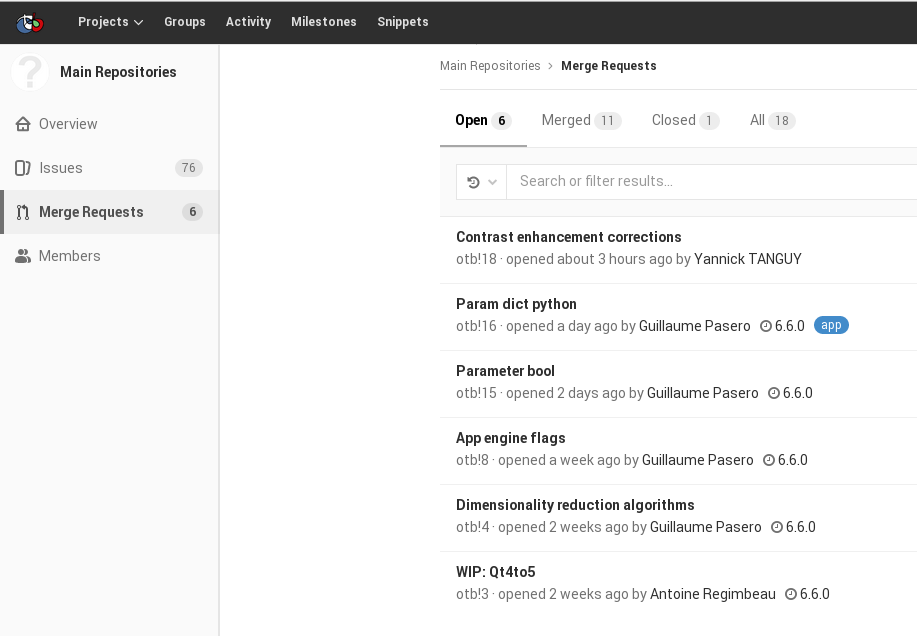
\includegraphics[width=\textwidth]{images/gitlab_mr.png}
    \end{columns}
\end{frame}


\vspace*{-6.5mm}
\begin{frame}[plain]
\hspace*{-11mm}
    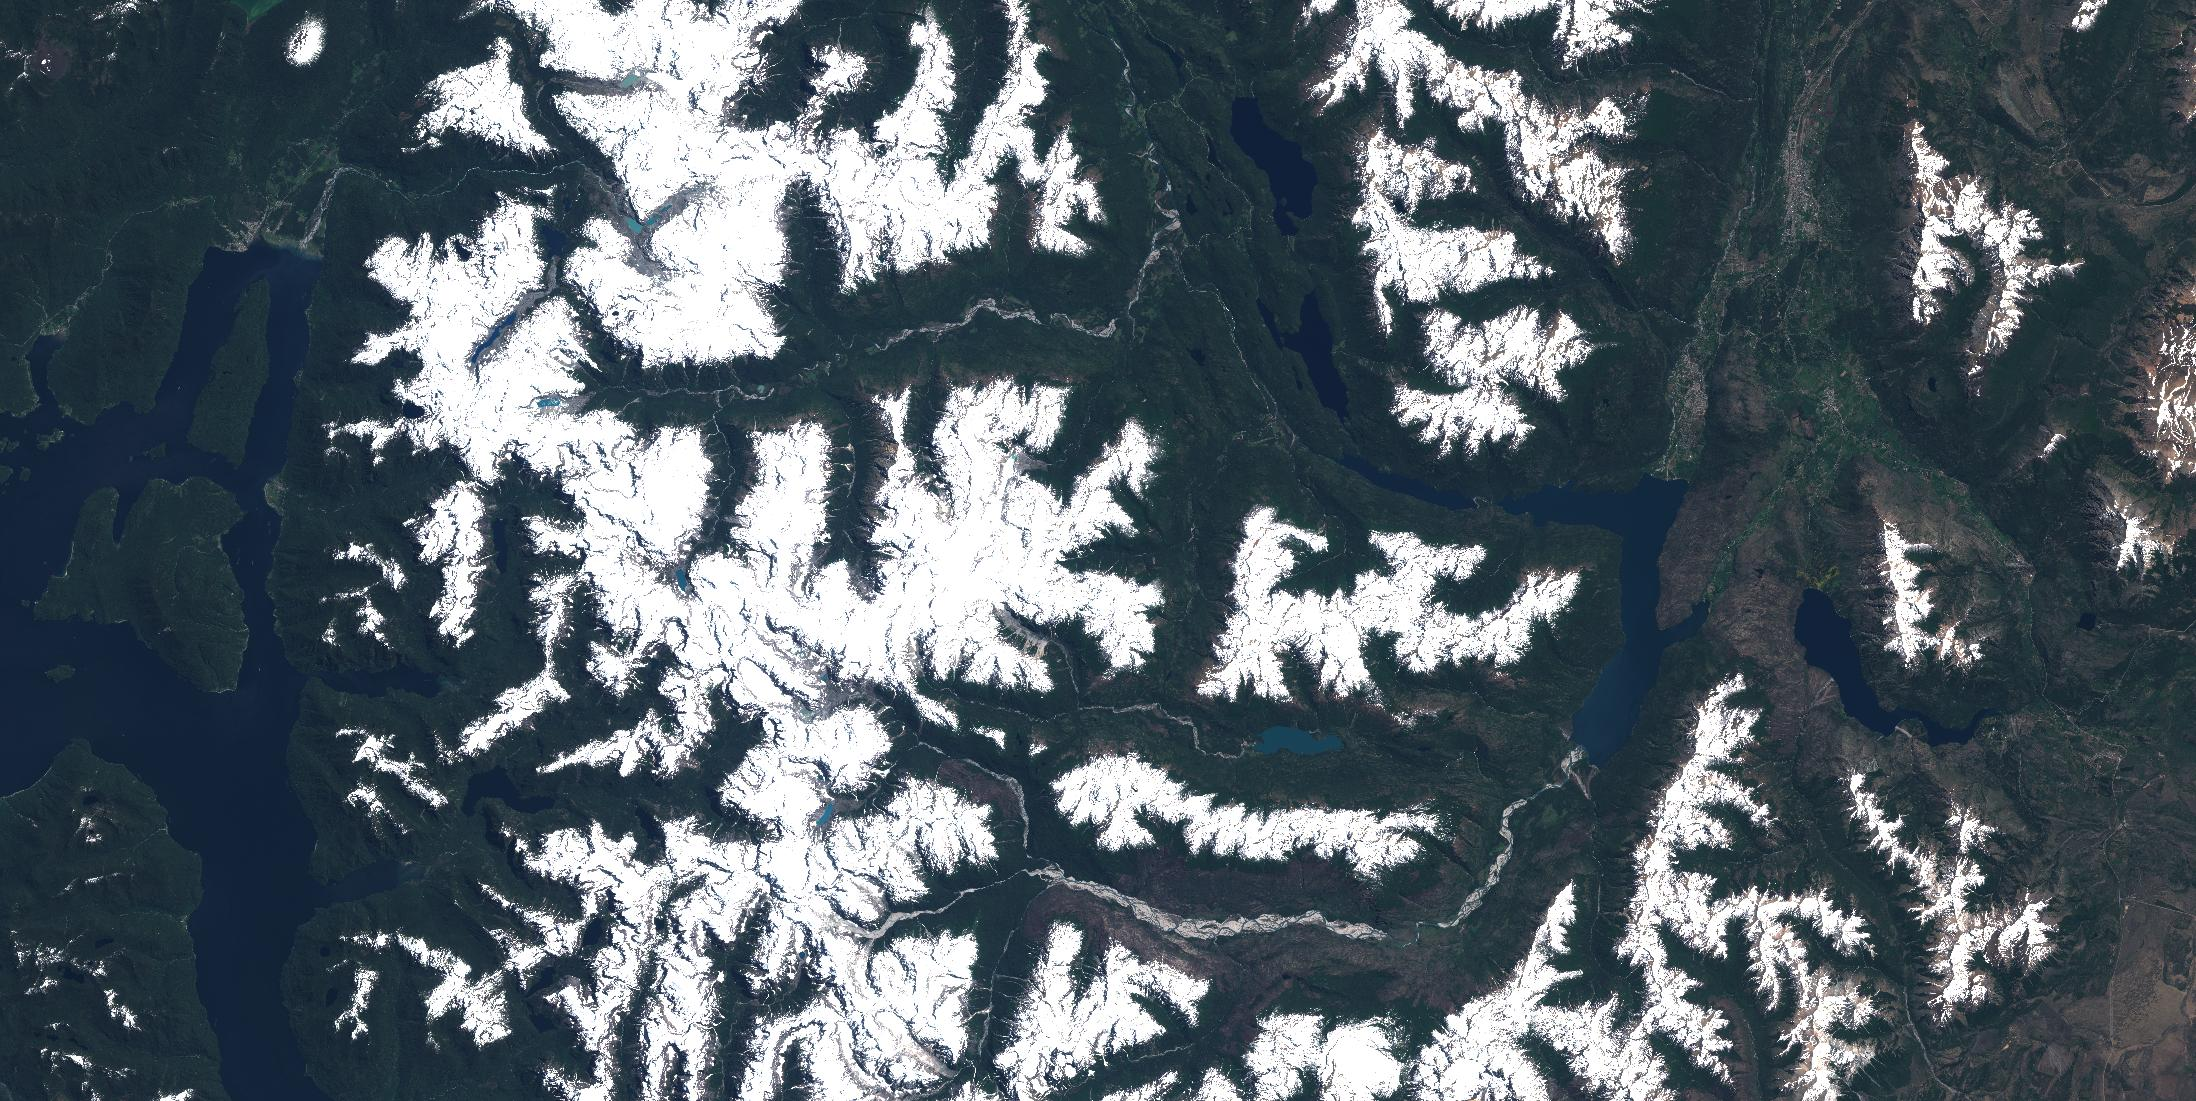
\includegraphics[keepaspectratio,height=1.1\paperheight]{images/imag4tci.jpg}
\end{frame}

\vspace*{-6.5mm}
\begin{frame}[plain]
\hspace*{-11mm}
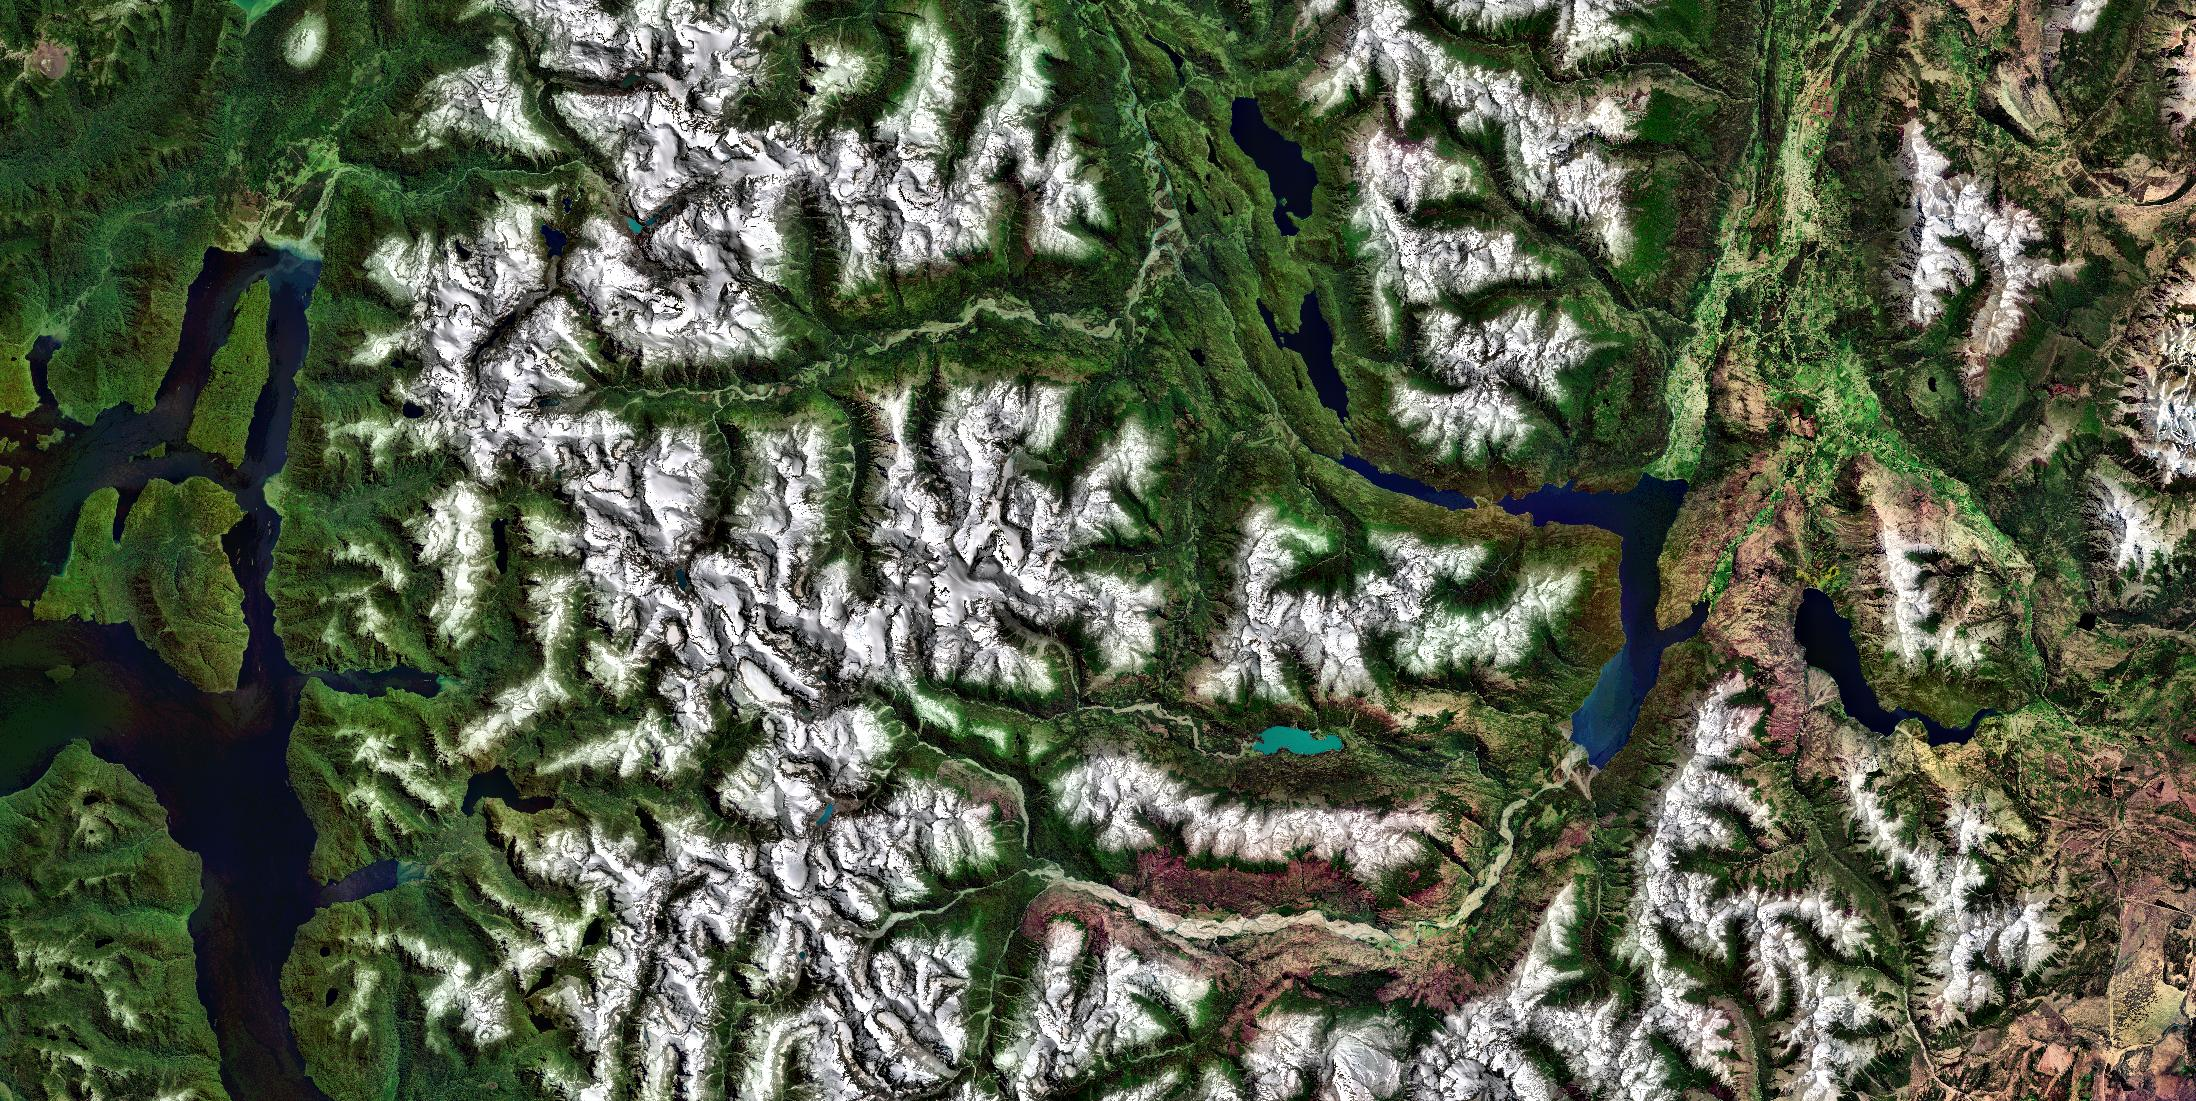
\includegraphics[keepaspectratio,height=1.1\paperheight]{images/image4_glob_each_lim20_8b_sub.jpg}
\end{frame}

\mode<all>
\begin{frame}
  \frametitle{6.6 (June 2018)}

  \begin{itemize}
  \item Data augmentation : generate synthetic samples to improve classifiers
    performances (CESBIO)
  \item New algorithms for dimensionality reduction : Autoencoders, PCA and Self
    Organizing Map (CESBIO)
  \item Multi writer (CS-SI)
  \end{itemize}  
\end{frame}


\begin{frame}[fragile]
  \frametitle{6.6 (June 2018)}
  \begin{itemize}
    \item Multi writer (CS-SI)
  \begin{lstlisting}[language=c++,breaklines=true,breakatwhitespace=true,frame =
      tb,framerule =
      0.25pt,fontadjust,backgroundcolor={\color{listlightgray}},basicstyle =
      {\ttfamily\tiny},keywordstyle =
      {\ttfamily\color{red}\textbf},identifierstyle = {\ttfamily},commentstyle =
      {\ttfamily\color{listcomment}\textit},stringstyle =
      {\ttfamily},showstringspaces = false,showtabs = false,numbers =
      none,numbersep = 2pt, numberstyle={\ttfamily\color{listnumbers}},tabsize =
      2]
  ReaderType1::Pointer reader1 = ReaderType1::New();
  reader1->SetFileName( inputImageFileName1 );

  ReaderType2::Pointer reader2 = ReaderType2::New();
  reader2->SetFileName( inputImageFileName2 );

  WriterType::Pointer writer = WriterType::New();
  writer->AddInputImage( reader1->GetOutput(), outputImageFileName1);
  writer->AddInputImage( reader2->GetOutput(), outputImageFileName2);
  writer->SetNumberOfLinesStrippedStreaming( numberOfLinesPerStrip );

  writer->Update();

  \end{lstlisting}
  \end{itemize} 
\end{frame}

\begin{frame}
  \frametitle{6.6 (June 2018)}
  \begin{itemize}
  \item Improvement in Application engine : simplify complex type  in input or
    output images (SAR images manipulation), stop button in the graphic interface...
  \item Migration from Qt4 to Qt5
  \item Better integration in QGIS (next slides)
  \item Lots of bugfixes!
  \end{itemize}  
\end{frame}


\section{OTB in QGIS}
%\mode<all>
%\section{Make OTB in QGIS Great Again!}

\begin{frame}
\frametitle{2009: OTB-QGIS plugin (Archeology)}
\begin{minipage}[t][6cm][t]{\textwidth}
\begin{center}
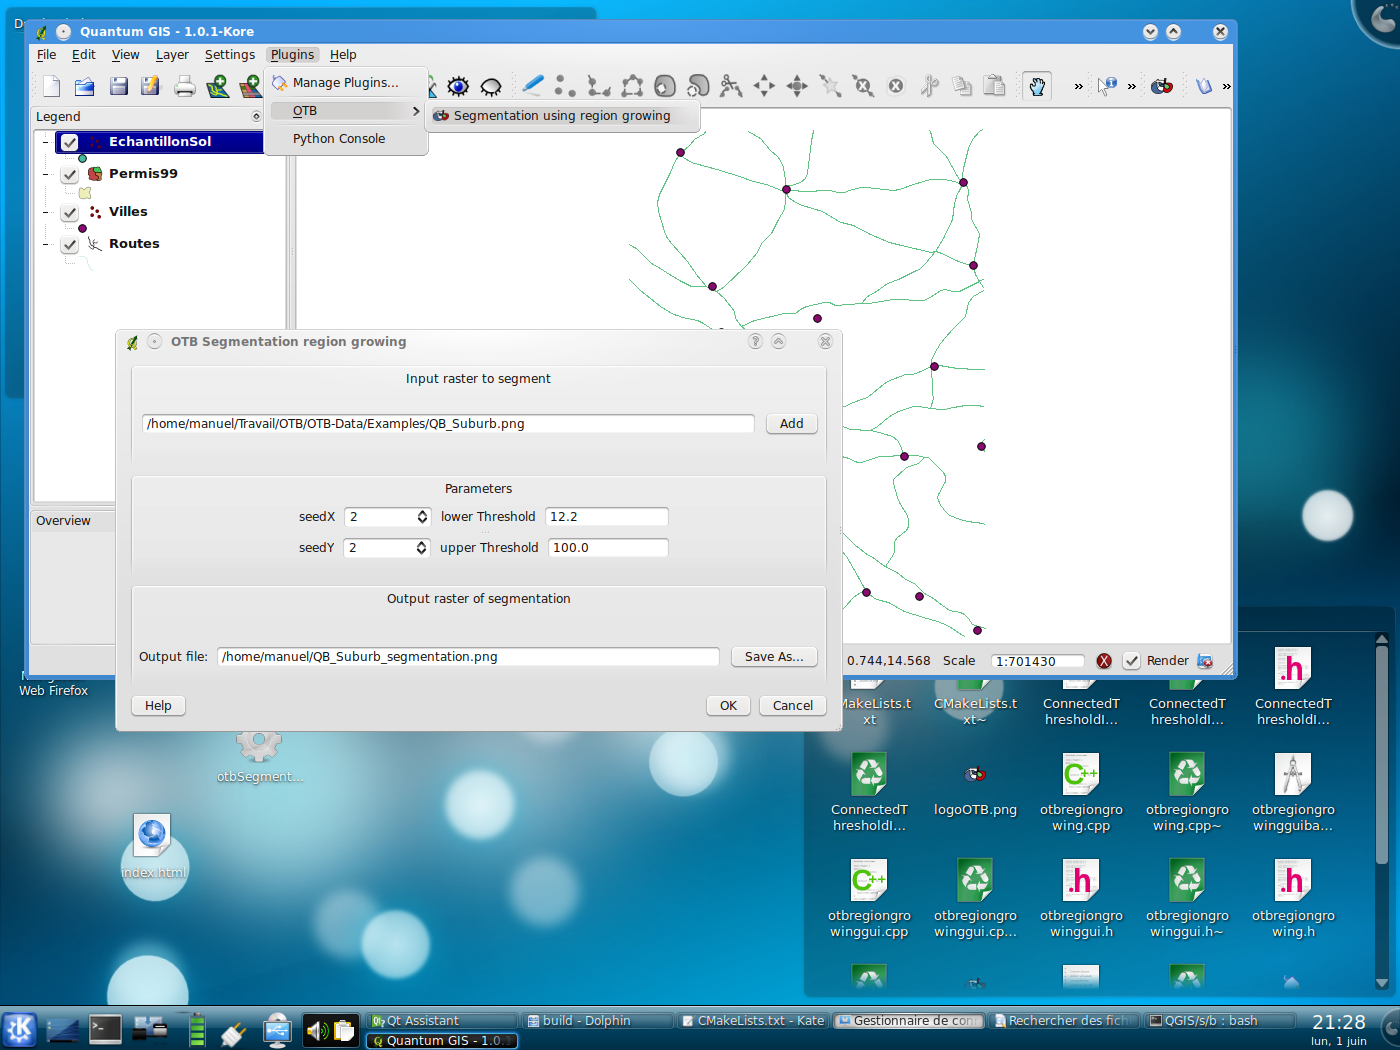
\includegraphics[width=0.7\textwidth]{images/otb-qgis-2009.png}
\end{center}
\end{minipage}
\end{frame}

\begin{frame}
\frametitle{2012-2017: First version of OTB plugin available in QGIS processing}
\begin{minipage}[t][6cm][t]{\textwidth}
\begin{center}
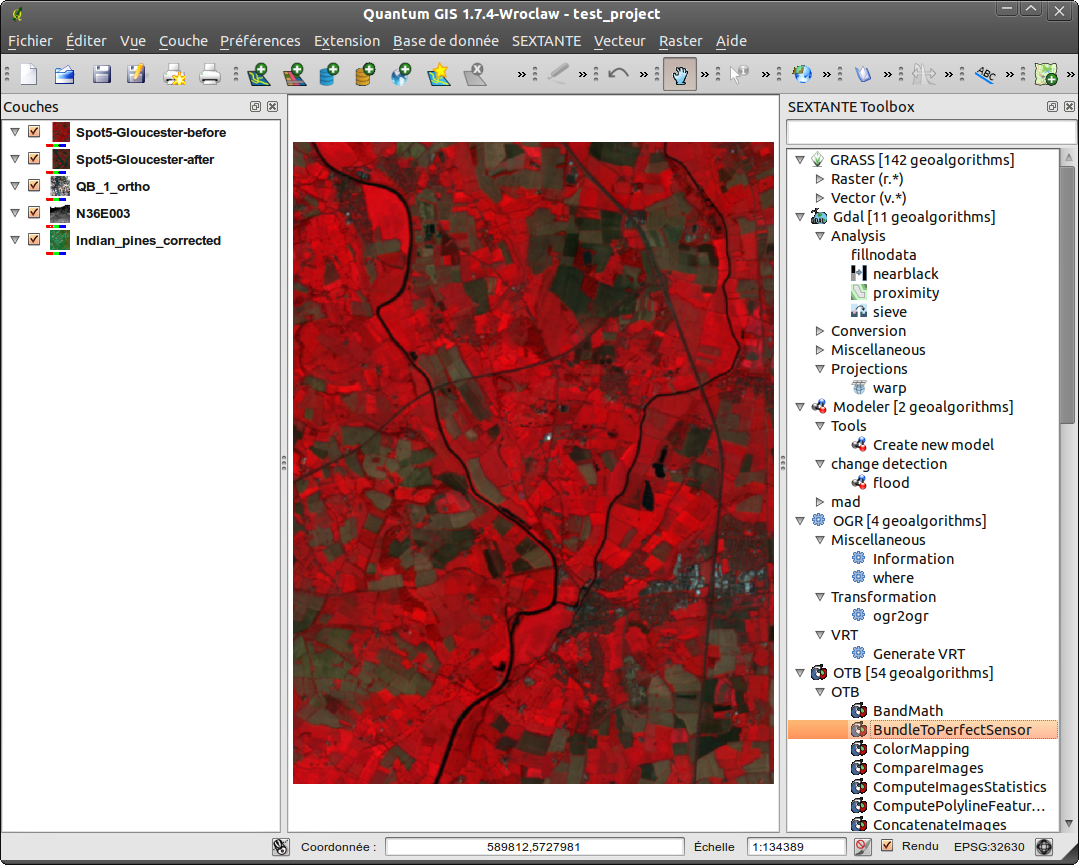
\includegraphics[width=0.7\textwidth]{images/otb_qgis.png}
\end{center}
\end{minipage}
\end{frame}

\begin{frame}
\frametitle{Access to OTB in QGIS: A powerful wedding}
\begin{itemize}
\item Facilitate access to OTB (QGIS widely use in the GIS community)
\item Avoid to duplicate efforts (use QGIS GUI, GIS features...)
\item Powerful features in QGIS processing (batch processing, Python scripting...)
\item Collaboration with the QGIS community is very positive
\item Support from QGIS developers
\item OSGeo \textit{power}
\item \href{https://www.youtube.com/watch?v=ufSQ2SgSIV4}{Demo}: \url{https://www.youtube.com/watch?v=ufSQ2SgSIV4}
\end{itemize}
\end{frame}

\begin{frame}
\frametitle{But everything is not that simple...}
\begin{itemize}
\item ``How to install and configure the last version of OTB in QGIS?''
\item ``Which versions of OTB is compatible with QGIS??''
\item ``Why I can't find the segmentation application in the QGIS processing panel?''
\item ``OTB applications seems to have slightly different names in QGIS?''
\item ``I give up OTB in QGIS...''
\item \alert{STOP!}
\item 2018: We need to improve the integration of OTB in QGIS
%\item Maintenance, Maintenance, Maintenance...
%\item Each version of otb needs to update list of descriptor files
%\item XML files which are hard to maintain.
%\item requires to update a blacklist and whitelist documents to list app that cannot be included and can be included
%\item needs manual update of these xml + followup on pull request
%\item works only with limited version of OTB (Not last release, mostly behind 3-4 releases)
%\item Nobody want to work on it from otb and qgis side. maintained by CS team
%\item Some applications were grouped, depending on their parameters : BinaryMorphologicalOperation (Closing, Dilate, Erode, Opening)
%\item Add new parameter in ParameterMultipleExternalInput processing, to use it in FusionOfClassifications
\end{itemize}

\end{frame}

\begin{frame}
  \frametitle{2018: OTB-QGIS plugin - Age of maturity :)}
  \begin{itemize}
    %\item Easy maintenance for both OTB team and QGIS team
  \item Keep It Simple
  \item Ease the integration of new versions of OTB in QGIS
    %\item Descriptors are generated, distributed and maintained by OTB
  \item Support of OTB binary installers in QGIS (``out of the box'')
  \item All OTB applications available in QGIS (same name, same documentation...)  
    %\item Out of box support for qgis via binary packages
    %\item Applications are not grouped.
    %\item Development took a turn due to some *non-technical*/politic issues in
    %qgis and otb
  \item \alert{Beta version} available as a plugin
  \item Hope the plugin will be soon added to QGIS source code
    %\item Will be added back to QGIS processing core later (Thanks to QGIS team)
    %\item Support for remote modules
    %\item OTB processing provider knows to recreate descriptor file for apps (if not found)
    %\item \alert{Version beta} disponible sous la forme d'un plugin
    % First version is distributed a plugin
  \item
    \href{https://gitlab.orfeo-toolbox.org/orfeotoolbox/qgis-otb-plugin}{https://gitlab.orfeo-toolbox.org/orfeotoolbox/qgis-otb-plugin}{Source
    code of the new plugin}
  \item Compatible with QGIS 3.2
  \item Thanks to all the QGIS team!
  \end{itemize}
\end{frame}

\begin{frame}
\frametitle{OTB configuration in QGIS}
\begin{center}
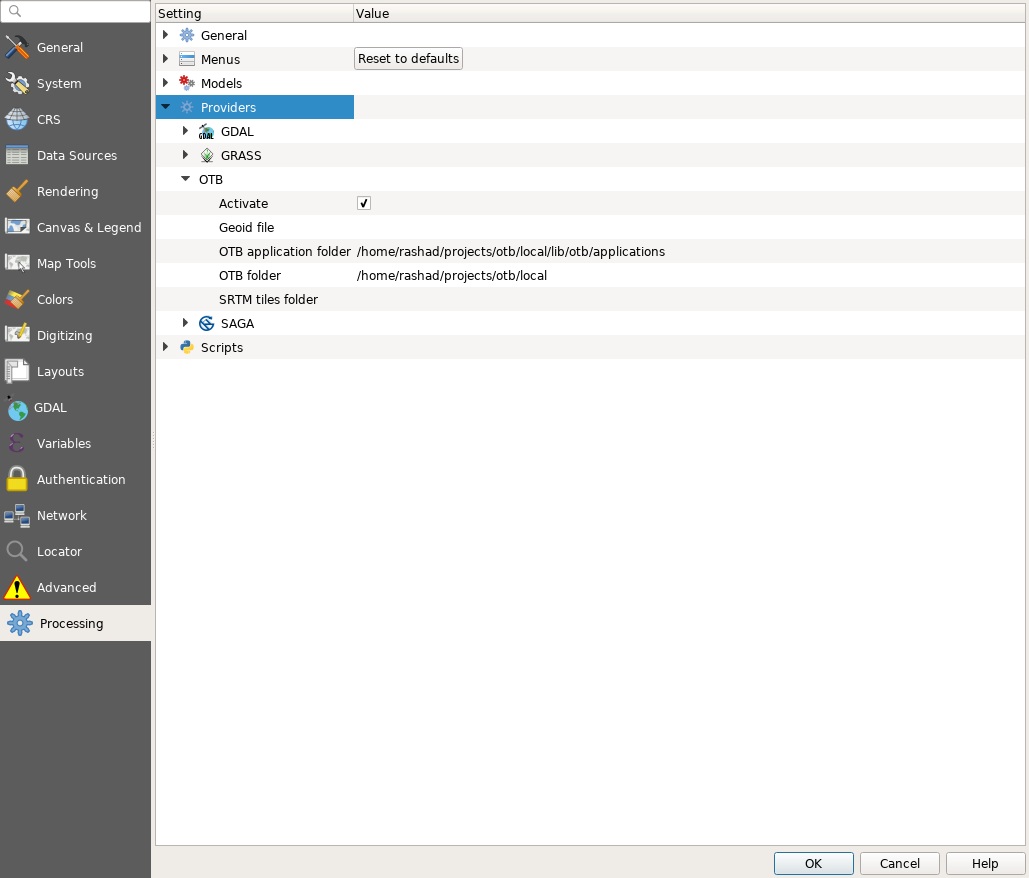
\includegraphics[width=0.8\textwidth]{images/qgis_otb_provider_config.png}
\end{center} 
\end{frame}

\begin{frame}
\frametitle{GUI of the \textit{Smoothing} application}
\begin{center}
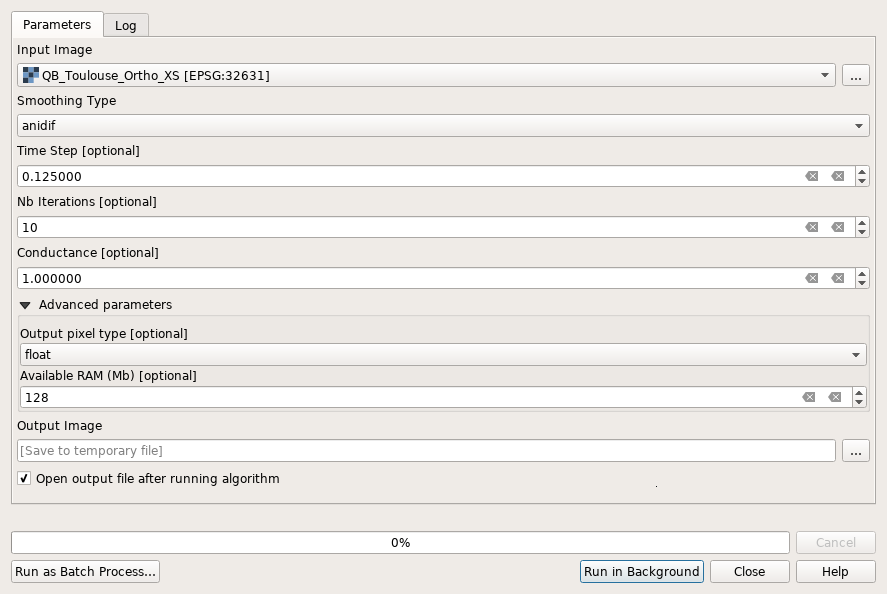
\includegraphics[width=0.8\textwidth]{images/qgis_smoothing.png}
\end{center} 
\end{frame}

\begin{frame}
\frametitle{GUI of the \textit{TrainImagesClassifier} application}
\begin{center}
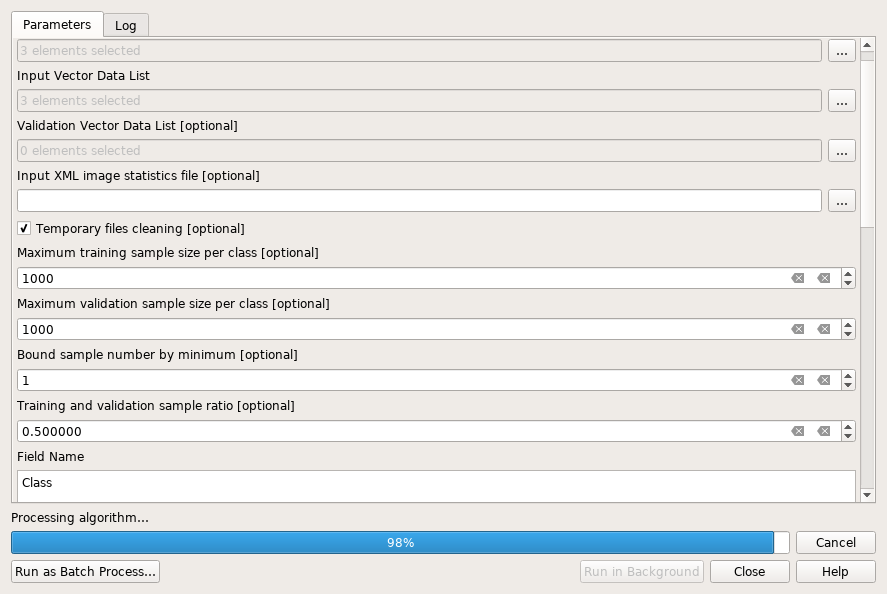
\includegraphics[width=0.8\textwidth]{images/qgis_train_classif.png}
\end{center} 
\end{frame}

\begin{frame}
\frametitle{Access to OTB in QGIS: A powerful wedding}
\begin{itemize}
\item Facilitate access to OTB (QGIS widely use in the GIS community)
\item Avoid to duplicate efforts (use QGIS GUI, GIS features...)
\item Powerful features in QGIS processing (batch processing, Python scripting...)
\item Collaboration with the QGIS community is very positive
\item Support from QGIS developers
\item OSGeo \textit{power}
\item \href{https://www.youtube.com/watch?v=ufSQ2SgSIV4}{Demo}: \url{https://www.youtube.com/watch?v=ufSQ2SgSIV4}
\end{itemize}
\end{frame}

\begin{frame}
  \frametitle{New OTB-QGIS plugin available!}
  \begin{itemize}
    %\item Easy maintenance for both OTB team and QGIS team
  \item Keep It Simple
  \item Ease the integration of new versions of OTB in QGIS
    %\item Descriptors are generated, distributed and maintained by OTB
  \item Support of OTB binary installers in QGIS (``out of the box'')
  \item All OTB applications available in QGIS (same name, same documentation...)  
    %\item Out of box support for qgis via binary packages
    %\item Applications are not grouped.
    %\item Development took a turn due to some *non-technical*/politic issues in
    %qgis and otb
  \item \alert{Beta version} available as a plugin
  \item Hope the plugin will be soon added to QGIS source code
    %\item Will be added back to QGIS processing core later (Thanks to QGIS team)
    %\item Support for remote modules
    %\item OTB processing provider knows to recreate descriptor file for apps (if not found)
    %\item \alert{Version beta} disponible sous la forme d'un plugin
    % First version is distributed a plugin
  \item
    Source code for new plugin: \url{https://gitlab.orfeo-toolbox.org/orfeotoolbox/qgis-otb-plugin}
  \item Compatible with QGIS 3.2
  \item Thanks to all the QGIS team!
  \end{itemize}
\end{frame}

\begin{frame}
\frametitle{OTB configuration in QGIS}
\begin{center}
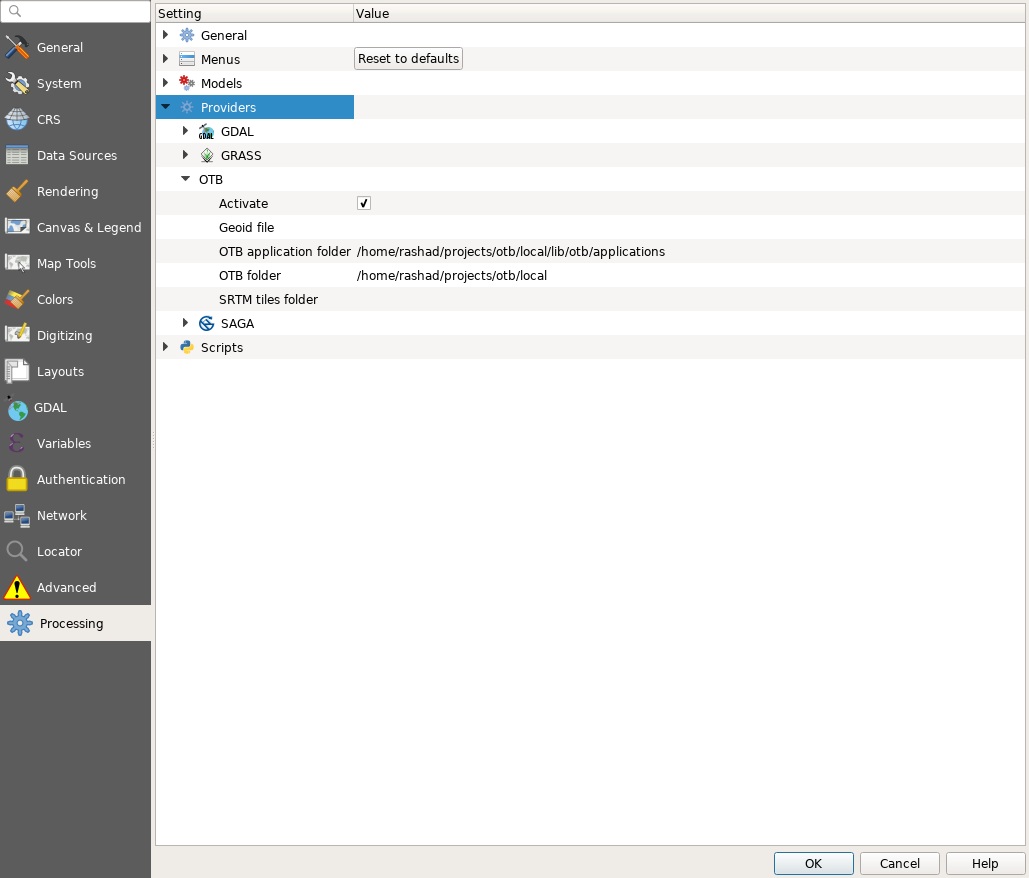
\includegraphics[width=0.8\textwidth]{images/qgis_otb_provider_config.png}
\end{center} 
\end{frame}

\begin{frame}
\frametitle{GUI of the \textit{TrainImagesClassifier} application}
\begin{center}
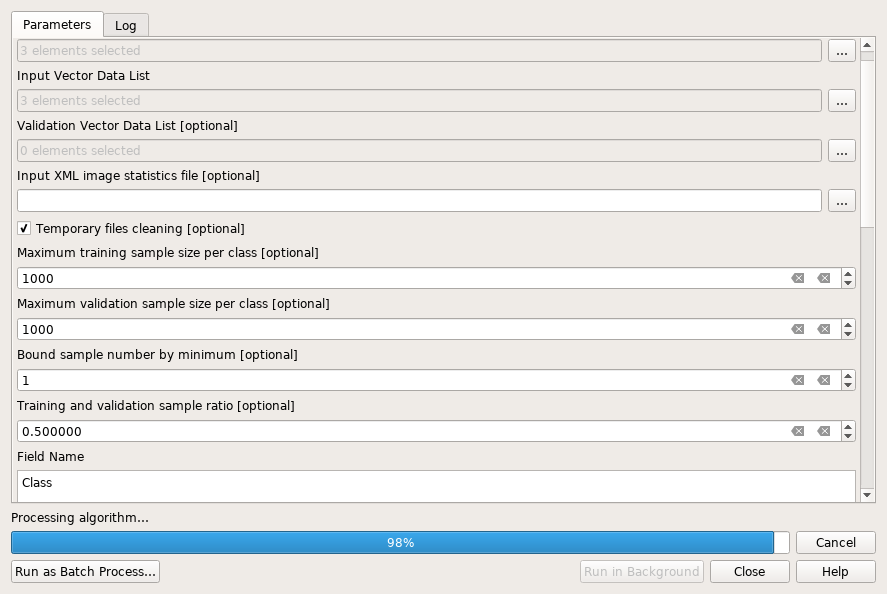
\includegraphics[width=0.8\textwidth]{images/qgis_train_classif.png}
\end{center} 
\end{frame}

\section{New remote modules}

\begin{frame}{About remote modules}
\begin{block}{What they are}
  \begin{itemize}
    \item Pieces of OTB code (filters, applications ...)
    \item That can be hosted on any git repository
    \item With a different licence
    \item While still being tested and packaged with OTB
    \item \url{gitlab.orfeo-toolbox.org/remote_modules/remote-module-template}
  \end{itemize}
\end{block}

\begin{block}{How people use them}
  \begin{itemize}
    \item A standard way to package new features to share with other
    \item Small modules (1 filter, 1 app) or bigger
    \item Processing chains in Python relying on one (or more) remote modules
    \end{itemize}
\end{block}  
\end{frame}

\subsection{Features as Remote Modules}

\begin{frame}{OTBTF remote module: OTB + tensorflow}
  \begin{itemize}
  \item Remote  module developed by Remi Cresson (IRSTEA)
  \item Based on TensorFlow
  \item Provides all the plumbing to perform Deep Learning based image processing on Remote Sensing images:
    \begin{itemize}
      \item Generate training data from the OTB training data sampling framework
      \item Train your network (can also be done directly with TensorFlow)
      \item Serve the model on full remote sensing images with streaming
    \end{itemize}
    \item \url{gitlab.irstea.fr/remi.cresson/otbtf}
  \end{itemize}
\begin{center}
  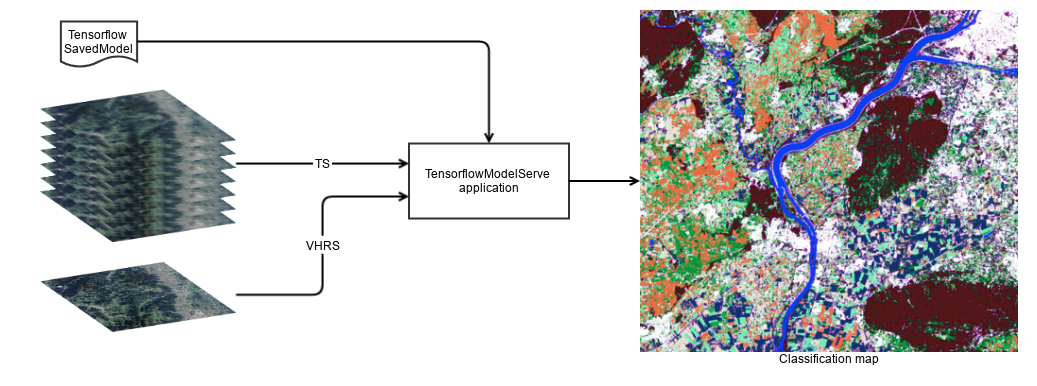
\includegraphics[width=0.8\textwidth]{images/classif_map.png}
\end{center}
\end{frame}

\section{More to come!}
\mode<all>
\begin{frame}
\frametitle{6.6.1 (soon!)}
\begin{block}{Bugfixes}
\begin{itemize}
\item Bugfix only release, 100\% backwards-compatible!
\item 50+ bugfixes backported from 7.0.0 milestone
\item Dependencies upgrades
\end{itemize}
\end{block}

\end{frame}


\mode<all>
\begin{frame}
\frametitle{7.0 (soon!)}
\begin{block}{Features}
\begin{itemize}
\item Documentation improvements
\item Many bug fixes
\item Add box kernel to morphological operations apps
\item No data extended filename for image writers
\end{itemize}
\end{block}

\begin{block}{Refactoring}
\begin{itemize}
\item Semantic Versioning (\url{https://semver.org})
\item \texttt{LSMSSmallRegionsMerging} -> \texttt{SmallRegionMerging}
\item Deprecate OTBMapnik and OTBVectorDataRendering
\item Convert -> DynamicConvert
\item Rename parameters, remove options...
\end{itemize}
\end{block}

\end{frame}


\begin{frame}
\frametitle{Support/Help/Contribute}
\vspace{-0.2cm}
\begin{block}{General resources}
\vspace{-0.2cm}
\begin{description}
\item[Site web] \href{http://www.orfeo-toolbox.org}{orfeo-toolbox.org}
\item[Wiki] \href{http://wiki.orfeo-toolbox.org}{wiki.orfeo-toolbox.org}
\item[Blog] \href{http://blog.orfeo-toolbox.org}{blog.orfeo-toolbox.org}
\end{description}
\end{block}
\vspace{-0.2cm}
\begin{block}{Documentation and help}
\vspace{-0.2cm}
\begin{description}
\item[Guides] Software Guide and CookBook (remote sensing recipes)
\item[Doxygen] \href{http://www.orfeo-toolbox.org/doxygen}{doxygen}
\item[Users mailing list] otb-users@googlegroups.com
\item[Developers mailing list] otb-developers@googlegroups.com
\end{description}
\end{block}
\vspace{-0.2cm}
\begin{block}{Follow-up}
\vspace{-0.2cm}
\begin{description}
\item[Look at the code?] \href{https://gitlab.orfeo-toolbox.org/orfeotoolbox/otb}{gitlab.orfeo-toolbox.org}
\item[Find a bug? Feature propositions?] \href{https://gitlab.orfeo-toolbox.org/orfeotoolbox/otb/issues}{gitlab.orfeo-toolbox.org/orfeotoolbox/otb/issues}
\item[Dashboard] \href{http://dash.orfeo-toolbox.org}{dash.orfeo-toolbox.org}
\end{description}
\end{block}
\end{frame}

\begin{frame}
  \frametitle{OSGeo and OSGeo-fr}
  \begin{block}{OSGeo}
    \vspace{-0.2cm}
    \begin{description}
    \item[OSGeo website] \href{https://www.osgeo.org/}{www.osgeo.org}
    \item[OSGeo-fr (French chapter)] \href{https://www.osgeo.asso.fr/}{osgeo.asso.fr}
    \end{description}
  \end{block}
  \vspace{-0.2cm}
  \begin{block}{Upcoming events (France)}
    \vspace{-0.2cm}
    \begin{description}
    \item[Capitole du Libre (17\&18 Nov)] \href{https://2018.capitoledulibre.org/}{2018.capitoledulibre.org}
    \item[Paris Open Source Summit (5\&6 Dec)] \href{https://www.opensourcesummit.paris/}{opensourcesummit.paris}
    \item[Rencontres des Utilisateurs Francophones de QGIS (13 \& 14 Dec)] \href{http://conf.qgis.osgeo.fr/}{conf.qgis.osgeo.fr}
    \end{description}
  \end{block}
  \vspace{-0.2cm}
  \begin{block}{FOSS4G}
    \vspace{-0.2cm}
    \begin{description}
    \item[FOSS4G 2019 Bucharest] \href{https://2019.foss4g.org/}{2019.foss4g.org}
    \end{description}
  \end{block}

\end{frame}

\begin{frame}
\frametitle{Survey by Inno3}
\begin{itemize}
\item Inno3 is currently conducting for CNES a study about open-source benefits
\item OTB is used as an example for this study
\item \color{red} They need your feedback! \color{red}
\end{itemize}

\begin{center}
  \begin{large}
    \url{https://huit.re/otb-survey}\\
    \vspace{0.5cm}
    Do not hesitate to discuss with them during the day \\
    \vspace{0.5cm}
    (Camille and Benjamin, raise your hands!)
    \end{large}
\end{center}

\end{frame}

\begin{frame}
\frametitle{Thank you! Any questions?}
\begin{minipage}[t][6cm][t]{\textwidth}
\begin{center}
\includegraphics[width=0.65\textwidth]{images/LOGOTB_blackbox.png}
\end{center}
\end{minipage}
\end{frame}


\end{document}
